\chapter{元编程}
\label{cp:meta}

\section{构建系统}

\textbf{构建系统是开发流程的基础}。其作用是\textbf{通过一系列规则和指令自动化地将源代码编译为可执行文件、库文件或者其他输出目标}。\textit{在小型项目中,手动编译和链接源文件可能已经足够,但是随着项目规模的增长,源文件之间的依赖关系变得错综复杂,手工编译不仅耗时耗力,还容易出错。}这时,构建工具便显得尤为重要。构建工具如\texttt{Makefile}和\texttt{CMake}可以自动处理文件依赖,编译、链接源文件,并支持跨平台的构建需求,使项目的开发流程更加高效和可靠。

\subsection{Makefile}

\textbf{Makefile是Linux系统中最早期且广泛使用的构建工具之一}。它依赖于\textit{GNU Make}工具,通过\textit{定义一组目标(target)、依赖关系(dependencies)和规则(rules),自动化地完成编译过程}。典型的\texttt{Makefile}文件通常由多个部分组成,描述了从源文件生成目标文件的过程。\\

我们只能给出一个简单的\texttt{Makefile}示例,如代码\ref{listing:makefile}所示。

\begin{longlisting}
    \begin{minted}{make}
CC = gcc
CFLAGS = -Wall -g

SRCS = main.c utils.c
OBJS = $(SRCS:.c=.o)
TARGET = program

$(TARGET): $(OBJS)
    $(CC) $(CFLAGS) -o $(TARGET) $(OBJS)

%.o: %.c
    $(CC) $(CFLAGS) -c $< -o $@

clean:
    rm -f $(OBJS) $(TARGET)
    \end{minted}
    \caption{Makefile编译C项目的示例}
    \label{listing:makefile}
\end{longlisting}

在这个Makefile中,\texttt{CC}表示\textit{编译器(此处为gcc)},\texttt{CFLAGS}定义了\textit{编译器的选项},包括显示所有警告(\texttt{-Wall})和生成调试信息(\texttt{-g})。\texttt{SRCS}列出了\textit{所有源文件},而\texttt{OBJS}则是由源文件生成的目标文件。\texttt{\$(TARGET)}是最终的可执行文件。\\

执行\texttt{make}命令,\texttt{Make}就会\textit{自动计算每个目标文件的依赖,并根据规则编译源代码}。clean命令用于清理生成的目标文件和可执行文件。\\

下面我们给出一个使用\texttt{Makefile}编译一个Hello World C程序的示例,如代码\ref{listing:makefile-example}所示。

\begin{longlisting}
    \begin{minted}{bash}
# 安装 make 工具
sudo apt install build-essential -y

# 假设目录中已有了 helloworld.c 文件
# 创建 Makefile 文件
echo 'CC=gcc
CFLAGS=-Wall -Wextra -std=c99

all: helloworld

helloworld: helloworld.c
	$(CC) $(CFLAGS) -o helloworld helloworld.c

clean:
	rm -f helloworld' >> Makefile

# 执行 make 命令
make
## 看到 gcc -Wall -Wextra -std=c99 -o helloworld helloworld.c 说明编译成功
chmod +x helloworld
./helloworld
## Hello, World!

# 清理编译文件
make clean
## rm -f helloworld 此时 helloworld 文件已被删除
    \end{minted}
    \caption{使用Makefile编译Hello World C程序}
    \label{listing:makefile-example}
\end{longlisting}

具体运行效果见图\ref{fig:makefile-example}。\\

\begin{figure}[!htbp]
    \centering
    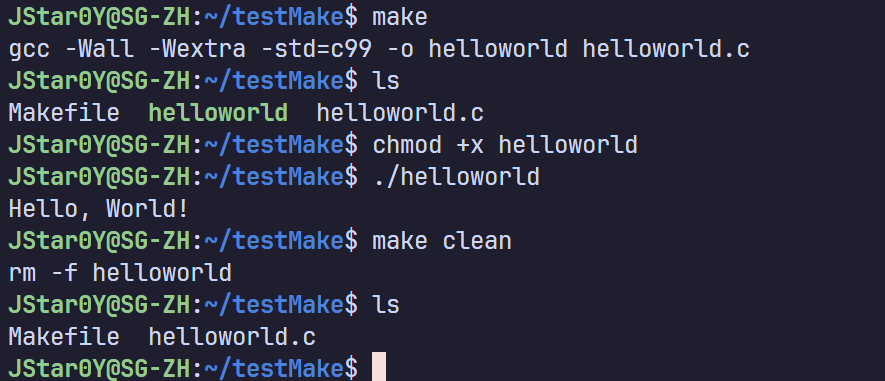
\includegraphics[width=0.8\textwidth]{Figures/make.png}
    \caption{使用Makefile编译Hello World C程序的运行效果}
    \label{fig:makefile-example}
\end{figure}

\textbf{Make的缺点显而易见。}虽然Makefile的简单、灵活和易于扩展使其在许多项目中被广泛使用。然而,\textbf{当项目变得更加复杂且跨平台需求增多时,Makefile的局限性开始显现。}特别是,当项目需要在不同的操作系统或编译器之间切换时,手动管理Makefile的复杂性变得不可控。